\documentclass[preprint]{sigplanconf}

\usepackage{amsmath}
\usepackage{amssymb}
\usepackage{alltt}
\usepackage{url}
\usepackage{natbib}
\usepackage{datetime}
\usepackage{graphicx}
\usepackage{comment}

%include polycode.fmt
%include play.fmt

% general stuff
\newcommand{\T}[1]{\texttt{#1}}
\newcommand{\C}[1]{\textsf{#1}}
\newcommand{\tup}[1]{\ensuremath{\langle #1 \rangle}}
\newcommand{\mtxt}[1]{\textsf{#1}}

\newcommand{\pic}[1]{\includegraphics[scale=0.55]{#1.eps}}

% examples
\newcounter{exmp}
\setcounter{exmp}{1}
\newcommand{\yesexample}{\subsubsection*{Example \arabic{exmp}}\addtocounter{exmp}{1}}
\newcommand{\noexample}{\hfill$\Box$}

\newcommand{\todo}[1]{\textbf{\textsc{Todo:} #1}}

% code blocks
\newenvironment{code}{\begin{alltt}\small}{\end{alltt}}
\newenvironment{codepage}
    {\begin{minipage}[h]{\textwidth}\begin{code}}
    {\end{code}\end{minipage}}

\newenvironment{example}{\yesexample}{\noexample}

\newcommand{\K}{\ensuremath{^\ast}} % kleene star
\newcommand{\D}{\ensuremath{\cdot}} % central dot

\renewcommand{\c}[3]{\tup{\T{#1},\T{#2},\T{\{#3\}}}}
\newcommand{\cc}[2]{\c{#1}{$\lambda$}{#2}}

\newcommand{\s}[1]{\ensuremath{_{\tt #1}}} % subscript, in tt font
\newcommand{\g}[1]{\{#1\}} % group, put { } round it
\newcommand{\U}{\textunderscore}
\newcommand{\vecto}[1]{\overrightarrow{#1\;}}
\newcommand{\gap}{\;\;}
\newcommand{\dom}{\text{dom}}

\newcommand{\derive}{\textsc{Derive}}

\newcommand{\compare}[2]{\subsubsection*{\textsf{#1} from #2:}\vspace{-1ex}}


\begin{document}

\conferenceinfo{Haskell Workshop '07}{date, City.} %
\copyrightyear{2007} %
\copyrightdata{[to be supplied]}

\titlebanner{\today{} - \currenttime{}}        % These are ignored unless
\preprintfooter{}   % 'preprint' option specified.

\title{Uniform Boilerplate and List Processing}
\subtitle{\textit{Or}: Scrap Your Scary Types}

\authorinfo{Neil Mitchell}
           {University of York, UK}
           {\url{http://www.cs.york.ac.uk/~ndm/}}
\authorinfo{Colin Runciman}
           {University of York, UK}
           {\url{http://www.cs.york.ac.uk/~colin/}}

\maketitle

\begin{abstract}
Generic traversals over recursive data structures are often referred to as \textit{boilerplate} code. The definitions of functions involving such traversals may repeat very similar patterns, but with variations for different data types and different functionality. While other generic traversal schemes have required extensions to the type system, this paper focuses on a conceptually simpler generic concept. The |Uniplate| class is introduced, which abstracts over common traversals and queries in a simple manner.
\end{abstract}

\section{Introduction}

Take a simple example of a recursive data type:

\begin{code}
data Expr  =  Val  Int
           |  Var  String
           |  Neg  Expr
           |  Add  Expr  Expr
           |  Sub  Expr  Expr
           |  Mul  Expr  Expr
           |  Div  Expr  Expr
\end{code}

The |Expr| type represents a small expression language for integer expressions, which permits free variables. Suppose we need to extract a list of all the variables in an expression:

\begin{code}
variables :: Expr -> [String]
variables (Var  x    ) = [x]
variables (Val  x    ) = []
variables (Neg  x    ) = variables x
variables (Add  x y  ) = variables x ++ variables y
variables (Sub  x y  ) = variables x ++ variables y
variables (Mul  x y  ) = variables x ++ variables y
variables (Div  x y  ) = variables x ++ variables y
\end{code}

This definition has the following undesirable characteristics:

\begin{itemize}
\item adding a new constructor would require an additional equation;
\item the |++| operation is specified many times;
\item the code is repetitive and uninteresting;
\item the code is unnecessarily long.
\end{itemize}

This problem is referred to as the \textit{boilerplate} problem. Using the library developed in this paper, the above example can be rewritten as:

\begin{code}
variables :: Expr -> [String]
variables x = [y | Var y <- everything x]
\end{code}

The type signature is optional, and would be inferred automatically if left absent. This example requires only Haskell 98. For more advanced examples we require multi-parameter type classes -- but no rank-2 types, functional dependencies or GADTs. The central idea is to make all operations work over a single \textit{uniform} type. By focusing on the simple case, we bring real benefits to the programmer.

\subsection{Contribution}

Ours is far from the first technique for `scrapping the boilerplate', the area has been researched extensively. But there are a number of novel features in our approach:

\begin{itemize}
\item We make use of \textit{list-comprehensions} \citep{wadler:list_comprehensions} for succinct queries.
\item We require \textit{no language extensions} for single-type traversals, and only multi-parameter type classes \cite{jones:mptc} for multi-type traversals.
\item Our \textit{choice of operations} is new: we shun some traditionally provided operations, and provide some uncommon operations.
\item We are able to implement our class on top of |Typeable| and |Data| \citep{lammel:syb}, making use of the built in compiler support if available.
\item We compare the \textit{relative performance} of traversal mechanisms, something that has been neglected in previous papers.
\end{itemize}

We have implemented all the techniques reported here. Our scheme requires less boilerplate than alternatives in almost all cases. We encourage readers to download the Uniplate library and try it out. It can be obtained from the website at \url{http://www.cs.york.ac.uk/~ndm/uniplate/}. A copy of the library has also been released, and is available on Hackage\footnote{\url{http://hackage.haskell.org/}}.

The ideas behind the Uniplate library have been used extensively, in both the Yhc compiler \cite{yhc} and the Catch tool \cite{me:catch_tfp}. In Catch there are over 100 Uniplate traversals.

\subsection{Road map}

\S\ref{sec:use_play} introduces the traversal combinators that we propose, along with short examples. \S\ref{sec:implement_play} discusses how these combinators are implemented in terms of a single primitive. \S\ref{sec:use_playex} extends this approach to multi-type traversals, and \S\ref{sec:implement_playex} covers the extended implementation. \S\ref{sec:properties} lists some properties of the functions in our library. \S\ref{sec:results} gives code comparisons to other examples, including the ``paradise'' benchmark, and performance measurements. \S\ref{sec:conclusion} makes concluding remarks and suggests directions for future work.


\section{Queries and Traversals}
\label{sec:use_play}

We define various queries and traversals, using the |Expr| type defined in the introduction as an example throughout. All the traversals rely on the class |Uniplate|, an instance of which is assumed for |Expr|. This instance and definition are covered in \S\ref{sec:implement_play}.

We use the term \textit{children} to refer to all maximal proper substructures of the same type. For example, |Add (Neg (Lit 1)) (Var "x")| has the children |Neg (Lit 1)| and |Var "x"|.

\subsection{Queries}

The Uniplate library provides a single method for implementing queries, the |universe| method.

\begin{code}
universe :: Play alpha => alpha -> [alpha]
\end{code}

This function takes a data structure, and returns a list of all data structures of the same type found within it. Imagining a data structure as a tree, |universe| returns the root of the tree, and all it's subtrees of the same type at all levels. For example:

\begin{code}
universe (Add (Neg (Var "x")) (Val 12)) =
    [Add (Neg (Var "x")) (Val 12)
    ,Neg (Var "x")
    ,Var "x"
    ,Val 12]
\end{code}

\begin{comment}
\begin{figure}
\pic{everything2}
\caption{Graphical representation of |everything|.}
\label{fig:everything}
\end{figure}

A visual representation of this example is given in Figure \ref{fig:everything}.
\end{comment}

One use of this mechanism for querying was given in the introduction. We have found that the pattern of using a list-comprehension to examine the results is common.

\begin{example}
Consider the task of seeing how many divisions by the literal 0 there are -- as this will cause a runtime error.

\begin{code}
countDivZero :: Expr -> Int
countDivZero x = length [() | Div _ (Val 0) <- everything x]
\end{code}
\end{example}

Note that we make essential use of the feature of list comprehensions that if a pattern does not match, then the item is skipped. In other syntactic constructs, failing to match a pattern results in a pattern-match error. Using the |universe| function, queries can be expressed very quickly and directly -- thanks to the power of Haskell's list processing.

\subsection{Bottom-up Traversals}

Another common operation covered by many boilerplate removal systems \cite{lammel:syb} is a function that makes modifications to every node in the data structure. We define as our standard traversal a bottom up traversal.

\begin{code}
traverse :: Play alpha => (alpha -> alpha) -> alpha -> alpha
\end{code}

\begin{example}
Suppose we wish to remove the |Sub| constructor assuming the equivalence:

\begin{code}
x - y == x + (- y)
\end{code}

To apply this rewrite at all possible places in the input expression we define:

\begin{code}
simplify x = traverse f x
    where  f (Sub x y)  = Add x (Neg y)
           f x          = x
\end{code}

This code can be read: apply the subtraction rule where you can, and where you cannot, do nothing. Adding additional rules is easy. Take for example:

\begin{code}
x + y = 2 * x       where x == y
\end{code}

Now we can add this new rule into our existing traversal:

\begin{code}
simplify x = traverse f x
    where  f (Sub x y)           = Add x (Neg y)
           f (Add x y) | x == y  = Mul (Val 2) x
           f x                   = x
\end{code}

Each equation corresponds to the natural Haskell translation of the rule. The |traverse| function manages all the required boilerplate.
\end{example}

So how does a bottom-up traversal work? The traversal starts by applying the function |f| to all the leaf nodes in the tree, then progressively working up to the root node. The condition on ordering is that before applying |f| to an expression, all the sub-expressions must have had |f| applied.

\subsection{Rewrite Traversals}

Besides bottom-up traversals, many boilerplate schemes would a top-down traversal (\cite{lammel:syb} has |everywhere'|). But if two traversals are defined, how should the user pick between them? Instead we focus on modelling traversals as rewrites -- showing why providing a top-down traversal is both unnecessary, and potentially dangerous! There is no barrier to defining a bottom-up traversal in our library, and we refer to such a hypothetical traversal as |traversal'|.

We define our rewrite traversal to be:

\begin{code}
rewrite :: Play alpha => (alpha -> Maybe alpha) -> alpha -> alpha
rewrite rule x = ...
\end{code}

A rewriting |rule| takes an expression of type |alpha|, and returns either |Nothing| to indicate that the rule is not applicable, or a |Just| indicating that a modification has been performed, and that the new expression should be checked for rewrites. The postcondition for |rewrite| is that there must be no places where |rule| could be applied. Another way of stating this is:

\begin{code}
forall r, x `o` all (isNothing . r) (universe (rewrite r x))
\end{code}

It is possible to define the |rewrite| function in terms of |traverse|:

\begin{code}
rewrite :: Play alpha => (alpha -> Maybe alpha) -> alpha -> alpha
rewrite f = traverse g
    where g x = maybe x (rewrite f) (f x)
\end{code}

This definition tries to apply the rule everywhere in a bottom-up manner. If at any point it makes a change, then the new tree has the rewrite applied to it. Assuming the set of rules is confluent and terminating, there will be no difference between a top-down and bottom-up application of the rules.

A disadvantage of |rewrite| is that if a rule modifies a tree only slightly, then large amounts of wasted work could be performed checking expressions repeatedly. Because of this, most programmers would rather use an explicit traversal -- namely top-down or bottom-up, and manage this rewriting themselves. But which one of top-down and bottom-up is most appropriate, and how would it be modified to ensure |rewrite| behaviour?

\subsubsection{Rewrite as Bottom-Up}
\label{sec:rewrite_bottom}

Given a rewrite |f :: alpha -> Maybe alpha|, we define the related function |f'| as follows:

\begin{code}
f' :: alpha -> alpha
f' x = maybe x id (f x)
\end{code}

What are the preconditions on |f| such that |forall x `o` rewrite f x == traverse f' x|? We can start by defining a more abstract representation of a rewrite rule:

\begin{code}
type Rewrite  = [(Tree,Tree)]
data Tree     = Branch String [Tree] | Leaf

f (Sub x y) = Add x (Neg y)
-- is represented by
[(Branch "Sub" [Leaf,Leaf],Branch "Add" [Leaf, Branch "Neg" [Leaf]])]
\end{code}

We can imagine |f| as a set of tree rewrite rules, where the tree on the left corresponds to the pattern matching, and the tree on the right corresponds to the generated value. We can now define the |equalBottomUp| function which returns True if a rewrite rule satisfies the property that |rewrite| and |traverse| give the same result:

\begin{code}
treeEq (Branch s1 t1) (Branch s2 t2) =
    s1 == s2 && zipWith treeEq t1 t2
treeEq _ _ = True

equalBottomUp :: Rewrite -> Bool
equalBottomUp rs =  not $ or  [treeEq a b | a <- map fst rs
                              ,b <- concatMap (everything . snd) rs]
\end{code}

If any of the generated values at any level overlaps with the root of any pattern match, then the traversal is not a rewrite. Taking the |simplify| traversal from from the previous section:

\begin{code}
f (Sub x y)           = Just $ Add x (Neg y)
f (Add x y) | x == y  = Just $ Mul (Val 2) x
f _                   = Nothing
\end{code}

Here |Add| occurs on the right-hand side of the first line, and on the left-hand side of the second. From this we can construct a value where the two alternatives differ:

\begin{code}
let x = Sub (Neg (Var "q")) (Var "q")

rewrite   f   x = Mul (Val 2) (Var "q")
traverse  f'  x = Add (Var "q") (Neg (Var "q"))
\end{code}

So is it possible to remedy this situation? Yes. Whenever the right-hand side introduces a new constructor, an additional onward call can be made:

\begin{code}
f' (Sub x y)           = f' $ Add x (f' $ Neg y)
f' (Add x y) | x == y  = f' $ Mul (f' $ Val 2) x
f' x                   = x
\end{code}

This approach guarantees that the traversal is a rewrite. In fact, only one |f'| application is necessary, the one attached to the construction of an |Add| value.


\subsubsection{Rewrite as Top-Down}

Now we pose the question: under what circumstances is a \textit{top-down} traversal a rewrite, and what modifications can be made to ensure it becomes so?

Before we can answer this question, we must first reflect on what a top-down traversal means. The usual answer \citep{lammel:syb} is that an operation is first applied at the root. The traversal is then applied recursively to each child of the (possibly transformed) root.

We can define the |equalTopDown| operation to test these the rewrite and top-down traversal for equivalence:

\begin{code}
equalTopDown rs =  not $ or  [treeEq a b | a <- map snd rs
                             ,b <- concatMap (everything . fst) rs]
\end{code}

The only change from |equalBottomUp| is that the |fst| and |snd| applications have been switched. Root values constructed on the right must not match anywhere on the left. Note that this restriction is neither more nor less severe than the one imposed on bottom-up traversals. For the |simplify| example, both produce the same result.

Is it possible to modify |f| minimally to permit a rewrite traversal? Yes. But the result is an encoding of bottom-up traversal. To see the full effect of the translation, we need a more complex example:

\begin{code}
f (Add (Lit x) (Lit y)  ) = Lit (x+y)
f (Mul (Lit 1) y        ) = y
\end{code}

\noindent becomes:

\begin{code}
f (Add x y) = case  (f x     , f y     ) of
                    (Lit x'  , Lit y'  ) -> Lit (x'+y')
                    _ -> Add x y
f (Mul x y) = case  f x of
                    Lit 1 -> f y
                    _ -> Mul x y
\end{code}

\noindent Or alternatively, making use of GHC's pattern-guards:

\begin{code}
f (Add  x y) | Lit x'  <- f x, Lit y' <- f y = Lit (x'+y')
f (Mul  x y) | Lit 1   <- f x = f y
\end{code}

We have both explicitly continued the execution \textit{before} performing a pattern match, and in the last branch where a leaf is returned, we explicitly continue \textit{afterwards}.

We consider top-down traversals to be more complex and less useful than bottom-up traversals, and we do not include them in our library. A previous version of our library did include top-down traversals, but we found they were rarely the correct choice. We discovered that most uses of top-down traversals were to model rewrites where information was pushed down, and it was easy to get the definition wrong in corner cases. This experience lead us to the decision that top-down traversals do not deserve library support. We include |rewrite| but suspect that most users would be better off using |traverse|, modified as described above.

\subsection{Action Traversals}

Rewrite traversals apply a set of rules \textit{repeatedly} until a fixed point is found. The alternative is an action traversal, where each node is visited and transformed \textit{once}. The |traverse| function can be used to perform this, but a standard technique is to thread a monad through the actions. We do this by introducing |traverseM|.

\begin{example}
Suppose we wish to rename each variable to be unique:

\begin{code}
uniqueVars :: Expr -> Expr
uniqueVars x = evalState (traverseM f x) vars
    where
        vars = ['x':show i | i <- [1..]]

        f (Var i)  = do  y:ys <- get
                         put ys
                         return (Var y)
        f x        = return x
\end{code}

Here a monadic computation is used. The program keeps track of the next item in the list to use, and replace the current item. Using the state monad, this can be done easily.
\end{example}

\subsection{Top-Down Descending}

Although top-down traversals are unnecessary for our library, we still believe that some traversals operate more naturally in a top-down manner. One extension to the top-down traversal pushes information downwards at the same time. We introduce the |descend| function, inspired by the Compos paper \cite{bringert:compos}.

\begin{code}
descend :: Play alpha => (alpha -> alpha) -> alpha -> alpha
\end{code}

The |descend| function applies a function to all children of a node, then reconstructs a new result using those results.

\begin{example}
Consider the addition of a constructor |Let String Expr Expr| -- binding the variable introduced. Now let us define a function |subst| to replace free variables with given expressions. In order to determine which variables are free, we need to ``remember'' variables that are bound as we descend. We can define |subst| as:

\begin{code}
subst :: [(String,Expr)] -> Expr -> Expr
subst rep x =
    case  x of
          Let name bind x -> Let name
              (subst rep bind)
              (subst (filter ((/= name) . fst) rep) x
          Var x -> fromMaybe (Var x) (lookup x rep)
          _ -> descend (subst rep) x
\end{code}
\end{example}


\subsection{Folds}

Traditionally in Haskell a fold replaces each constructor with an alternative \todo{ref}. To define a complete fold on a data type, each constructor must be represented -- giving boilerplate problems once more. We define a fold which provides a default operation:

\begin{code}
fold :: Play alpha => ([r] -> t) -> (alpha -> t -> r) -> alpha -> r
fold combine operate = ...
\end{code}

This fold takes two functional arguments: |combine| takes a value representing each child of an expression, and combines them into a token |t|; |operate| takes a token representing the children of a node, along with the node itself, into a result |r|.

\begin{example}
Imagine that |Expr| programmers are paid by the \textit{depth of expression} they produce:

\begin{code}
depth :: Expr -> Int
depth = fold (foldr max 0) $ const (+1)
\end{code}

Here we have used |foldr max 0| to combine all the children -- |maximum| is inappropriate, as |maximum [] = {-"\bot"-}|. The second function |const (+1)| simply adds one to the previous depth.
\end{example}

Our choice of fold operator seems a little unusual at first. One might have expected only one functional argument. We can define such a fold, and implement |depth| in terms of it:

\begin{code}
foldId :: Play alpha => (alpha -> [r] -> r) -> alpha -> r
foldId = fold id

fold combine operate = foldId (\a b -> operate a (combine b))

depth = foldId (foldr max 0 . map (+1))
\end{code}

This function is a perfectly common pattern, although by having a slightly more general version we allow more boilerplate to be removed in some examples -- particularly when some constructors require different operations.

\begin{example}
Give a slightly better example which shows why you need the more general version.
\end{example}


\subsection{EverythingContext}

The final operation in the library is a curious one -- we have not seen it referenced in any other library, even in those which attempt to include all variations \cite{ren:generic_recursion_toolbox}. However, if the user requires this particular function, they really do need it -- faking it from other operations requires a lot of monadic complexity. This function was actually contributed by a user, which we feel enhances our claim that average users can construct their own operations upon our framework.

Imagine that you wish to change the value of \textit{a single} literal by 1, either increasing or decreasing. This particular operation could be useful for mutation testing. To do this we provide the function:

\begin{code}
everythingContext :: Play alpha => alpha -> [(alpha, alpha -> alpha)]
\end{code}

This function returns two lists, one of which is the list as would be returned by everything. The other is the function which would replace the hole which the given expression was removed from. It has the properties:

\begin{code}
forall x `o` everything x == map fst (everythingContext x)
forall x `o` all (== x) [b a | (a,b) <- everythingContext x]
\end{code}

Now we are able to easily write our function:

\begin{code}
mutants :: Expr -> [Expr]
mutants x =  [gen (Val j)
             | (Val i, gen) <- everythingContext x
             , j <- [i-1, i+1]]
\end{code}


\subsection{Summary}

\begin{figure}
\begin{code}
module Data.Generics.Play where

class Play alpha where
    descend            :: (alpha -> alpha) -> alpha -> alpha
    descendM           :: Monad m => (alpha -> m alpha) -> alpha -> m alpha
    everything         :: alpha -> [alpha]
    everythingContext  :: alpha -> [(alpha, alpha -> alpha)]
    fold               :: ([r] -> t) -> (alpha -> t -> r) -> alpha -> r
    rewrite            :: (alpha -> Maybe alpha) -> alpha -> alpha
    rewriteM           :: Monad m  => (alpha -> m (Maybe alpha))
                                   -> alpha -> m alpha
    traverse           :: (alpha -> alpha) -> alpha -> alpha
    traverseM          :: Monad m => (alpha -> m alpha) -> alpha -> m alpha
\end{code}
\caption{All |Play| methods.}
\label{fig:play}
\end{figure}

We present all our methods in Figure \ref{fig:play}, including several monadic variants. We consider these methods encapsulate most of the common operations. In our experience, the most common operations are |everything| and |traverse|, followed by |traverseM| and |descend|.


\section{Implementing the |Play| class}
\label{sec:implement_play}

Requiring each class to implement nine separate methods would be overly arduous. Instead we implement all of these operations on top of just a single method:

\begin{code}
replaceChildren :: Play alpha => alpha -> ([alpha], [alpha] -> alpha)
replaceChildren x = (children,generate)
\end{code}

Given |x|, the function |replaceChildren| will return a tuple comprising of: |children| - all the children of the same type; |generate| - a function to generate a new value with a different set of children. The caller of |generate| must ensure that the length of the list given to it is the same as the length of |children|. The implementor of |replaceChildren| must ensure two conditions:

\begin{code}
forall x `o` x == generate children
    where (children,generate) = replaceChildren x

forall x ys `o`  length ys == length children =>
                 fst (replaceChildren (generate ys)) == ys
    where (children,generate) = replaceChildren
\end{code}

Firstly, generating a new value using the existing children must give the same value back. Secondly, after inserting a new set of children, getting those children must return them back.


\subsection{Operations in terms of |replaceChildren|}

Defining operations in terms of |replaceChildren| is easy, we implement the four most common as an example. None is more than a handful of lines long, and none has great deep complexity:

\begin{code}
everything :: Play alpha => alpha -> [alpha]
everything x = x :
    concatMap everything $ fst $ replaceChildren x

traverse :: Play alpha => (alpha -> alpha) -> alpha -> alpha
traverse f x = f $ generate $ map (traverse f) current
    where (current, generate) = replaceChildren x

traverseM :: (Monad m, Play alpha) => (alpha -> m alpha) -> alpha -> m alpha
traverseM f x = mapM (traverseM f) current >>= f . generate
    where (current, generate) = replaceChildren x

descend :: Play alpha => (alpha -> alpha) -> alpha -> alpha
descend f x = generate $ map f current
    where (current, generate) = replaceChildren x
\end{code}

The common pattern is to call replace children, then perform some action on the current children, before combining them back. Writing additional traversals with different properties can be done in a similar manner. The |everything| function may be optimised further -- something we return to in \S\ref{sec:optimise_everything}.

\subsection{Writing |Play| instances}
\label{sec:play_instances}

\begin{figure}
\begin{code}
instance Play Expr where
    replaceChildren (Neg  a    )  = ([a]    , \[a']     -> Neg  a'     )
    replaceChildren (Add  a b  )  = ([a,b]  , \[a',b']  -> Add  a' b'  )
    replaceChildren (Sub  a b  )  = ([a,b]  , \[a',b']  -> Sub  a' b'  )
    replaceChildren (Mul  a b  )  = ([a,b]  , \[a',b']  -> Mul  a' b'  )
    replaceChildren (Div  a b  )  = ([a,b]  , \[a',b']  -> Div  a' b'  )
    replaceChildren _             = ([]     , \[]       -> x           )
\end{code}
\caption{Instance of |Play| for |Expr|.}
\label{fig:play_expr}
\end{figure}

We construct a |Play| instance for the |Expr| type in Figure \ref{fig:play_expr}. The pattern of the instance can be seen easily. The default clause has no children of type |Expr|, meaning the leaves have been reached.

The distinguishing feature of our library is that the children are defined in terms of their type. While this feature keeps the queries and traversals simple, it does mean that the instance definition is dependent on the types of the constructors. We now describe the derivation rules, followed by information on the \derive{} tool that performs this task automatically. By optionally making use of Multi-Parameter Type Classes we are able to eliminate some of this complexity, see \S\ref{sec:implement_playex}.


\subsection{Derivation Rules}

In order to model the derivation of an instance, it is necessary to have a model of the types that are being manipulated:

\begin{code}
type Name  = String
type Var   = String

data Data  = Data Name [Var] [Ctor]
data Ctor  = Ctor Name [Type]
data Type  = TyPrim | TyVar Var | TyApp Data [Type]
\end{code}

When writing a |Play| instance for a particular data type, |isTarget| will return True for that data type. We can define how to produce a function for each |Data| type that is used, using the |_D| function:

\begin{code}
_D (Data name vars ctors) = unwords $
    ['d':name] ++ vars ++ ["x ="]
    ["case x of {"] ++
        separate ";" (map _C ctors) ++
    ["}"]

_C (Ctor name typs) =
    [name] ++ vars ++ [" -> "] ++
    ["unit"] ++ [name] ++
    separate "<>" (zipWith (:) vars (map _T typs)) ++
    where vars = ['v':show i | i <- [1..length typs]]

_T (TyPrim       ) = ["unit"]
_T (TyVar  v     ) = [v]
_T (TyApp  d ts  )
    | isTarget d  = ["target"]
    | otherwise   = ['d':dataName d] ++ map _T ts

separate sep xs = concat $ intersperse [sep] xs
\end{code}

Using this derivation, the |Expr| type comes out as:

\begin{code}
dExpr x = case x of
    Val  v1     -> unit Val  <> unit v1
    Var  v1     -> unit Val  <> dList unit v1
    Neg  v1     -> unit Neg  <> target v1
    Add  v1 v2  -> unit Add  <> target v1 <> target v2
    Sub  v1 v2  -> unit Sub  <> target v1 <> target v2
    Mul  v1 v2  -> unit Mul  <> target v1 <> target v2
    Div  v1 v2  -> unit Div  <> target v1 <> target v2

dList a x = case x of
    []          -> unit []
    (:)  v1 v2  -> unit (:) <> a v1 <> dList a v2
\end{code}

This derivation now provides sufficient information for use to define |replaceChildren| in several ways. If we are willing to limit ourselves to target types which have no type arguments. The simplest way is to define:

\begin{code}
instance Play Expr where
    replaceChildren x = (getChildren x, setChildren x)
\end{code}


\subsubsection{|getChildren|}

Now we can define |getChildren| as:

\begin{code}
getChildren x = dExpr x

unit    = const []
target  = (:[])
(<>)    = (++)
\end{code}

From these definitions we can do some reasoning. For example, |dList| is equivalent to |concatMap|. From this property, we can see that |concatMap (const [])| is equivalent to |const []|. This information can be used to simplify some instances.

\subsubsection{|setChildren|}

We can define |setChildren| as:

\begin{code}
setChildren x = value (dExpr x)

type Cont t = [alpha] -> (t,[alpha])

unit :: t -> Cont t
unit x ns = (x,ns)

target :: alpha -> Cont alpha
target x (n:ns) = (n,ns)

value :: Cont t -> [alpha] -> t
value c ns = fst $ c ns

(<>) :: Cont (a->b) -> Cont a -> Cont b
(<>) a b ns1 =  let  (a'  ,ns2  ) = a  ns1
                     (b'  ,ns3  ) = b  ns2
                in   (a' b',ns3)
\end{code}

While this derivation does provide the correct instances, we can improve the simplification opportunities and runtime speed by moving to continuations:

\begin{code}
type Cont t = [alpha] -> (t -> [alpha] -> r) -> r

unit    x  ns      c  = c x ns
target  x  (n:ns)  c  = c n ns
value   c  ns         = c ns const

(<>) a b ns c =  a  ns $ \a'  ns ->
                 b  ns $ \b'  ns ->
                 c (a' b') ns
\end{code}

\subsection{Using Derive}

Applying the presented derivation rules is quite time consuming, and is itself a form of boilerplate -- albeit one specific for each type. The DrIFT tool \cite{drift} is well known for defining instances which can be constructed purely from the information contained in type definition. However, there are limitations to the DrIFT tool -- it is unable to operate with the presence of certain Haskell extensions, and requires a separate pre-processing stage on all compilers.

As a separate project, we have developed the \derive{} tool \cite{derive}, in collaboration with Stefan O'Rear. We have extended \derive{} to allow seamless derivation of the |Play| instance. The tool is based on Template Haskell \cite{template_haskell}, but allows Haskell code to be generated which can be appended to the current file.

Taking an example:

\begin{code}
data Term  =  Name String
           |  Apply Term [Term]
              deriving ( {-! \textsf{Play} !-} )
\end{code}

When running the \derive{} tool over this file, the generated code is:

\begin{code}
instance Play Term where
    replaceChildren (Name x1) =
        ([], \_ -> Name x1)

    replaceChildren (Apply x1 x2) =
        (x1:x2, \(n:ns) -> Apply n ns)
\end{code}

This code follows from the definition, but \derive{} has special mechanisms to optimise out redundant patterns to produce cleaner code. If the user of \derive{} wishes, they can take advantage of the Template Haskell support in GHC by writing:

\begin{code}
$( derive makePlay {-"\;{}^{\prime\prime}"-}Term)
\end{code}

The use of \derive{} removes the need for a user to understand the rules to create an instance of the |Play| class.


\section{Multi-type Queries and Traversals}
\label{sec:use_playex}

We have introduced |Play| which operates on values of type |Expr|. Now let us imagine that |Expr| is merely the expression type in a language with statements:

\begin{code}
data Stmt  =  Assign    String  Expr
           |  Sequence  [Stmt]
           |  If        Expr    Stmt Stmt
           |  While     Expr    Stmt
\end{code}

We can define a |Play| instance for |Stmt|, and perform queries and traversals upon it. However, we may run into limitations. Consider the task of extracting all literals from within a |Stmt| -- this task is not possible with |Play|.

The |Play| class takes a value of type |alpha|, and operates on its children of type |alpha|. What we now require is something that takes a value of type |beta|, but operates on the children of type |alpha| within it -- we call this class |PlayEx|. Typically the type |beta| will be a container of |alpha|. We can extend our operations by specifying how to find the |alpha|'s within the |beta|'s, and then perform the standard Play operations upon the |alpha|. In the above example, our |alpha| would be |Expr|, and our |beta| would be |Stmt|.

We first introduce |PlayOn|, which requires an explicit function to move between the |alpha| and |beta|. Next we make use of MPTC's to generalise this function into a type class, named |PlayEx|.

\subsection{The |PlayOn| Operations}

We define a set of operations, including |everythingOn| and |traverseOn|, which take an additional argument from the standard |Play| operators. We call this additional argument |replaceType|, which describes how to move from the containing type (|beta|) to the contained type (|alpha|).

\begin{code}
type ReplaceType beta alpha = beta -> ([alpha], [alpha] -> beta)
replaceType :: ReplaceType beta alpha
\end{code}

The semantics of |replaceType| are that starting from |beta|, the function should return the highest children in the tree of type |alpha|. This particular requirement means that if |alpha == beta| the root node should be returned:

\begin{code}
replaceType :: ReplaceType alpha alpha
replaceType x = ([x], [x'] -> x')
\end{code}

We can now define |everythingOn| and |traverseOn| which take an explicit |replaceType| function:

\begin{code}
everythingOn :: Play to => ReplaceType beta alpha -> beta -> [alpha]
everythingOn replaceType x =
    concatMap everything $ fst $ replaceType x

traverseOn ::  Play to => ReplaceType beta alpha ->
               (alpha -> alpha) -> beta -> beta
traverseOn replaceType f x =
    generate $ map (traverse f) current
    where (current, generate) = replaceType x
\end{code}

These operations are similar to the original |everything| and |traverse|. The functions unwrap the |beta| to find the |alpha|, operate using the standard |Play| operations upon the |alpha|, then rewrap if necessary.

Passing the |replaceType| argument is a little tedious -- a much better approach would be to encapsulate this in a type class, and have it passed as a dictionary argument. Alas this requires MPTC's, which we wish to avoid just slightly longer.

By making a simplifying assumption, we are able to achieve slightly more elegant code, abstracting away the |replaceType| argument. Take for example the Yhc.Core library, part of the York Haskell Compiler (Yhc), which makes use of |Play|. In this library, the central types, along with which types they include, are:

\begin{code}
data Core      =  Core String [String] [CoreData] [CoreFunc]

data CoreFunc  =  CoreFunc String String CoreExpr

data CoreExpr  =  CoreVar   String
               |  CoreApp   CoreExpr  [CoreExpr]
               |  CoreCase  CoreExpr  [(CoreExpr, CoreExpr)]
               |  CoreLet   [(String, CoreExpr)] CoreExpr
               |  ...
\end{code}

Most queries and traversals are performed on the |CoreExpr| type, however it is often convenient to start from one of the other types. Take for example the |coreSimplify| operation -- it simplifies expressions, but may be called upon one individual expression, a function, or a program. If we are willing to freeze the type of |alpha| as |CoreExpr| we can write a class:

\begin{code}
class  PlayExpr beta where
       replaceTypeExpr :: ReplaceType beta CoreExpr

everythingExpr  = everythingOn replaceTypeExpr
traverseExpr    = everythingOn replaceTypeExpr

instance PlayExpr Core where ...
instance PlayExpr CoreFunc where ...
instance PlayExpr CoreExpr where ...
instance PlayExpr beta => PlayExpr [beta] where ...
\end{code}

This technique has been used in the Yhc compiler. The Yhc compiler is written in Haskell 98 to allow for bootstrapping, which requires the restriction to single-parameter type classes.

\subsection{The |PlayEx| class}

If we are willing to make use of the MPTC extension, we can define a class |PlayEx| which includes the |replaceType| function.

\begin{code}
class  PlayEx beta alpha where
       replaceType :: ReplaceType beta alpha
\end{code}

This takes us outside the realm of Haskell 98, however we feel that the MPTC is conceptually simple to understand. We have not required functional dependencies, and our code is all able to execute on both Hugs and GHC.

We can now implement |everythingEx| and |traverseEx| in terms of their |On| counterparts:

\begin{code}
everythingEx  :: PlayEx beta alpha => beta -> [alpha]
everythingEx  = everythingOn replaceType

traverseEx    :: PlayEx beta to => (alpha -> alpha) -> beta -> beta
traverseEx    = traverseOn replaceType
\end{code}

We now present two examples from \S\ref{sec:use_play}, but implemented using |PlayEx|. These operations will now work on |Expr|, |Stmt| or many other types -- being strictly more general than the previous versions.

\begin{code}
variables :: PlayEx beta Expr => beta -> [String]
variables x = [y | Var y <- everythingEx x]
\end{code}

The |variables| example from before requires only one change: the addition of the |Ex| suffix to |everything|. The type signature has changed so that instead of |Expr -> [String]| we have replaced |Expr| with |PlayEx beta Expr => beta|. Another way of looking at this is instead of requiring the input to be an |Expr|, we merely require that from the input we know how to reach an |Expr|.

\begin{code}
simplify x = traverseEx f x
    where  f (Sub x y)  = Add x (Neg y)
           f x          = x
\end{code}

With |simplify| we have again made one single change: the addition of |Ex| at the end of |traverse|. In general the move to |PlayEx| requires few code changes, merely the use of the new set of |Ex| functions.

\section{Implementing PlayEx}
\label{sec:implement_playex}

The complicating feature of |replaceType| is that when defining |PlayEx| where |alpha == beta| the program does not descend to the children, but simply returns this particular node. This ``same type'' restriction can be captured either using the type system, or using |Typeable|. We present three methods for defining a |PlayEx| instance -- offering a trade-off between performance, compatibility and volume of code. The first method, Manual, requires $O(n^2)$ instances but is the highest performance and fewest extensions. The second method makes use of the |Typeable| class providing reasonable speed with $O(n)$ instances and no further Haskell extensions. The final method makes use of the |Data| class, providing fully automatic instances with GHC, but requiring the use of rank-2 types, and performing the slowest. All methods can be fully automated using \derive{}, and provide a simplified method for writing |Play| instances.

The |PlayEx| class is a nice abstraction, which is independent of the method used to implement the instances. This abstraction allows the user to start with the simplest instance scheme available to them, allow a move to alternative schemes afterwards, to gain increased performance and compatibility.

\subsection{Manual instances}

Writing manual instances requires the |Data.Generics.PlayManual| module to be imported. This style requires a maximum of $n^2$ instance definitions, where $n$ is the number of types which contain each other, but gives the highest performance and most type-safety. These instances still depend on the type of each field, but are easier to define than the |Play| instance discussed in \S\ref{sec:play_instances}. An example for |Expr| would be:

\begin{code}
instance PlayOne Expr where
    playOne x =
        case x of
            Neg  a    -> play Neg  |* a
            Add  a b  -> play Add  |* a |* b
            Sub  a b  -> play Sub  |* a |* b
            Mul  a b  -> play Mul  |* a |* b
            Div  a b  -> play Div  |* a |* b
            _         -> play x
\end{code}

This module provides four combinators -- | ||*|, | ||+|, | ||-| and | ||||*| to indicate the structure of the field to the right. The | ||*| combinator says that the value on the right is of the target type, | ||+| says that the target type is contained within the value, | ||-| says that the target type is not in the value, and | ||||*| says that the value to the right is a list of the target type. We use the law that |play f ||- x| is equivalent to |play (f x)| to obtain the definition presented above.

This style of definition naturally expands to the multi-type traversal, for example:

\begin{code}
instance PlayAll Stmt Expr where
    playAll x =
        case x of
            Assign    a b    -> play Assign    |-  a |*  b
            Sequence  a      -> play Sequence  |+  a
            If        a b c  -> play If        |*  a |+  b |+ c
            While     a b    -> play While     |*  a |+  b
\end{code}

Note that in these two examples we have defined |PlayOne| and |PlayAll|. From these definitions the library can infer |Play| and |PlayEx| with the appropriate semantics. The information we have provided with | ||-| and | ||+| can be used to direct the search more precisely -- cutting out redundant exploration down branches that do not have the target type. The use of | ||||*| is an optimisation which allows the list to be directly manipulated with |replaceChildren| -- instead of producing and consuming the list twice.

This approach requires increasingly large number of definitions, one for container/contained pair. While this has the potential of reaching $n^2$, in reality this is rarely the case. Often very specific traversal pairs will dominate, and only those actually invoked by the code need to specified. The restricted number of type classes also gives increased type safety -- instance such as |PlayEx Expr Stm| do not exist, so this error can be eliminated.

We have named this approach ``Manual'' even though it makes full use of library provided primitives to structure the instances. The reason for referring to this as manual is that the person (or tool) writing the instances must be aware of the types -- not simply applying syntactic rules. In our experience these combinators offer similar performance to hand-tuned instances, see \S0 for measurements.


\subsection{In terms of |Typeable|}

Instead of writing $O(n^2)$ classes to capture the notion of which target is being looked for, we can use the |Typeable| class to test at runtime whether we have reached the target type. We again present derivations much as before, based on the combinators | ||+| and | ||-|:

\begin{code}
instance (Typeable a, Play a) => PlayAll Expr a where
    playAll x =
        case x of
            Neg a    ->  play Neg  |+ a
            Add a b  ->  play Add  |+ a |+ b
            Sub a b  ->  play Sub  |+ a |+ b
            Mul a b  ->  play Mul  |+ a |+ b
            Div a b  ->  play Div  |+ a |+ b
            _        ->  play x

instance (Typeable a, Play a) => PlayAll Stm a where
    playAll x =
        case x of
            Assign    a b    -> play Assign    |-  a |+ b
            Sequence  a      -> play Sequence  |+  a
            If        a b c  -> play If        |+  a |+ b |+ c
            While     a b    -> play While     |+  a |+ b
\end{code}

This module provides no | ||*| combinator -- these instances have no notion of which type we are searching for, so could not possibly answer as to whether it had been found. The | ||+| combinator is the most common, continuing the traversal. However, if we were to use | ||+| when the right-hand value was an |Int|, or other primitive type we did not wish to examine, we would require a |PlayAll| definition for |Int|. To omit these unnecessary instances, we can use | ||-| to indicate that the type is not of interest.

The |Data.Generics.PlayTypeable| module is able to automatically infer |PlayEx| instances given a |PlayAll|. Alas this is not the case for |Play|. Instead we must manually write:

\begin{code}
instance Play Expr where
    replaceChildren = replaceChildrenAll

instance Play Stmt where
    replaceChildren = replaceChildrenAll
\end{code}

At this point the reader may wonder why we cannot automatically infer this?

\begin{code}
instance PlayAll alpha alpha => Play alpha where
    replaceChildren = replaceChildrenAll
\end{code}

Consider the |Expr| type. To infer |Play Expr| we require an instance for |PlayAll Expr Expr|. To infer this instance we require |Typeable Expr| (trivial) and |Play Expr| -- which we are already in the process of inferring! This requires co-inductive or recursive dictionaries -- something that GHC has, but which Hugs does not. To allow continuing compatibility with Hugs, and the use of fewer extensions, we require the user to write these explicitly for each type.


\subsection{In terms of |Data|}
\label{sec:implement_playdata}

We are able to make use of the existing |Data| and |Typeable| instances provided by the SYB approach to define the necessary classes. To have access to all |Play| and |PlayEx| instances simply:

\begin{code}
import Data.Generics
import Data.Generics.PlayData

data Expr  = ... \? \? deriving (Typeable, Data)
data Stmt  = ... \? \? deriving (Typeable, Data)
\end{code}

The disadvantages of this are the lack of type safety - you can now do entirely meaningless operations, which the earlier definitions would have spotted as being an error. This code will also only work where Data.Generics is supported, namely GHC at the present time\footnote{Hugs supports the required rank-2 types for |Data.Generics|, but the work to port the library has not been done yet.} The clear advantage is that there is almost no work to creating Play instances.

\begin{figure}
\begin{code}
repChildren  :: (Data alpha, Play beta, Typeable alpha, Typeable beta)
             => alpha -> ([beta],[beta] -> alpha)
repChildren item = (collect, generate)
    where
        collect = concat $ gmapQ getChildrenEx item

        generate xs = evalState (gmapM f item) xs
        f x = do  let (col,gen) = replaceChildrenEx x
                  (as,bs) <- liftM (splitAt $ length col) get
                  put bs
                  return $ gen as
\end{code}
\caption{Code for |Play| in terms of |Data|.}
\label{fig:playdata}
\end{figure}

How do we implement these classes? The fundamental operation is given in Figure \ref{fig:playdata}. The |repChildren| function descends to each of the child nodes, and is guarded by a |Typeable| cast to ensure that |alpha /= beta|. The operation to get the children can be done using |gmapQ|. The operation to replace the children is more complex, requiring a state monad to keep track of the items to insert.

This instance is not optimised for speed, in particular the |splitAt|/|length| portion will take traverse the list more than is necessary. We discuss how to come up with an optimised version in \S\ref{sec:optimise_playdata}.


\section{Properties}
\label{sec:properties}

\todo{Prove or at least QuickCheck these properties! I am unsure if this section is worth keeping.}

This section discusses various properties that hold. Some of these could be turned into GHC optimisation rules, but this has not been done.

\subsection{Identity Properties}

These properties refer to which operations have which units. We have ignored the issue of strictness in the following examples:

\begin{code}
descend   id == id
traverse  id == id
rewrite   (const Nothing) == id

descendM   return == return
traverseM  return == return
rewriteM   (return . const Nothing) == return

fold _ const = id
\end{code}

\subsection{Combination Properties}

These properties relate to the combination of traversals.

\begin{code}
everything x = fold concat (:)
-- everything . traverse f == map (traverse f) . everything
-- does not hold!
\end{code}

We are unaware of any other properties that hold.

\subsection{List Properties}

A list is defined inductively as |data [alpha] = [] || alpha : [alpha]|. We can therefore define a |Play| instance as:

\begin{code}
instance Play [alpha] where
    replaceChildren []      = ([]    , const []       )
    replaceChildren (x:xs)  = ([xs]  , \[xs] -> x:xs  )
\end{code}

Now some common list operations can be represented as traversals:

\begin{code}
everything == tails
\end{code}

We can also define a |PlayEx| instance as:

\begin{code}
instance Play alpha => PlayEx [alpha] alpha where
    replaceType xs = (xs, id)
\end{code}

In which case we have the following properties, where the list instance is being used:

\begin{code}
traverseEx  f == map f
descendEx   f == map f
everythingEx == id
\end{code}


\section{Results and Evaluation}
\label{sec:results}

There are two distinct ways to evaluate a boilerplate reduction scheme, firstly by the amount of boilerplate it removes, and secondly by the runtime performance. We consider the first metric to be the most important, but also the hardest to measure. We first give a set of nine example programs, written using Play, SYB and Compos operations. We then benchmark all these operations and present the results.

\subsection{Boilerplate Reduction}
\label{sec:results_boilerplate}

To choose a representative set of benchmarks we have taken the first three examples from this paper, three from the Compos paper, and the three given in the SYB paper termed the ``Paradise Benchmark''. In all cases the Compos, SYB and Play functions are denoted by a preceding module name. In some instances, a single operate function can be written the same in both SYB and Play -- where this is possible we have done so. Where possible, type signatures have been left absent -- these are a form of boilerplate that Haskell already deals with.

\subsubsection{The Play Paper}

\compare{variables}{Play}

\begin{code}
Play.variables x = [y | Var y <- everything x]

SYB.variables = everything (++) ([] `mkQ` f)
    where  f (Var y)  = [y]
           f _        = []

Comp.variables :: Expr a -> [String]
Comp.variables x = case x of
    Var y -> [y]
    _ -> composOpFold [] (++) variables x
\end{code}

In this example only Compos has been given a type signature, in the other examples one can be automatically inferred -- but not for Compos due to the use of GADT's. We note that list comprehensions allow for succinct queries.

\compare{zeroCount}{Play}

\begin{code}
Play.zeroCount x = length [() | Div _ (Val 0) <- everything x]

SYB.zeroCount = SYB.everything (+) (0 `mkQ` f)
    where  f (Div _ (Val 0))  = 1
           f _                = 0

Comp.zeroCount :: Expr a -> Int
Comp.zeroCount x = case x of
    Div y (Val 0) -> 1 + zeroCount y
    _ -> composOpFold 0 (+) zeroCount x
\end{code}

Here the Play solution does not feel as neat as it could, the list of |()| is inelegant. However, Play is the only scheme that is able to use the standard |length| function, the other two have expressed the operation as a fold. The Compos solution requires additional boilerplate, to explicitly continue the operation on |Div y| -- which may be easy to overlook.

\compare{simplify}{Play}

\begin{code}
simp (Sub x y)           = simp $ Add x (Neg y)
simp (Add x y) | x == y  = Mul (Val 2) x
simp x                   = x

Play.simplify = traverse simp

SYB.simplify = everywhere (mkT simp)

Comp.simplify :: Expr a -> Expr a
Comp.simplify x = case x of
    Sub  a b -> simplify $ Add (simplify a) (Neg (simplify b))
    Add  a b -> case  (simplify a, simplify b) of
                      (a',b')  | a' == b'   -> Mul (Val 2) a'
                               | otherwise  -> Add a' b'
    _ -> composOp simplify x
\end{code}

We have used a modified version of |simplify| discussed in \S\ref{sec:rewrite_bottom}, which ensures that the two rules are applied everywhere possible. This situation requires a bottom-up traversal, which Compos does not provide, and so addition boilerplate is required.

\subsubsection{Multi-type traversals from Compos}

\begin{figure}
\begin{code}
data Stm  =  SDecl    Typ Var
          |  SAss     Var Exp
          |  SBlock   [Stm]
          |  SReturn  Exp

data Exp  =  EStm  Stm
          |  EAdd  Exp Exp
          |  EVar  Var
          |  EInt  Int

data Var  =  V String

data Typ  =  T_int | T_float
\end{code}
\caption{Data type from Compos.}
\label{fig:compos}
\end{figure}

The statement type manipulated by the Compos paper are given in Figure \ref{fig:compos}. The Compos paper translates this type into a GADT, while Play and SYB both accept the definition as supplied.

We have not discussed the |warnAssign| function from the Compos paper, as it could be implemented much more neatly as a query, rather than a monadic fold. We cover the remaining three functions.

\compare{rename}{Compos}

\begin{code}
ren (V x) = V ("_" ++ x)

Play.rename = traverseEx ren

SYB.rename = everywhere (mkT ren)

Comp.rename :: Tree c -> Tree c
Comp.rename t = case t of
    V x -> V ("_" ++ x)
    _   -> composOp rename t
\end{code}

The first thing to note is the Play function is shorter, there is only one constructor in type |Var|. In contrast Compos has merged all constructors into one GADT, and can not benefit from this knowledge.


\compare{symbols}{Compos}

\begin{code}
Play.symbols x = [(v,t) | SDecl t v <- everythingEx x]

SYB.symbols = everything (++) ([] `mkQ` f)
    where  f (SDecl t v)  = [(v,t)]
           f _            = []

Comp.symbols :: Tree c -> [(Tree Var, Tree Typ)]
Comp.symbols x = case x of
    SDecl t v -> [(v,t)]
    _ -> composOpMonoid symbols t
\end{code}

Here the Compos function does a traversal of the tree, however again the Play class simply extracts the right bits. The use of lists again benefits Play over SYB.

\compare{constFold}{Compos}

\begin{code}
optimise (EAdd (EInt n) (EInt m)) = EInt (n+m)
optimise x = x

Play.constFold = traverseEx optimise

SYB.constFold = everywhere (mkT optimise)

Comp.constFold :: Tree c -> Tree c
Comp.constFold e = case e of
    EAdd x y -> case  (f x, f y) of
                      (EInt n, EInt m) -> EInt (n+m)
                      (x',y') -> EAdd x' y'
    _ -> composOp constFold e
\end{code}

The constant folding operation is a bottom-up traversal, requiring sub expressions to have been replaced before they are examined. Unfortunately Compos only supports top-down traversals, requiring the user to manually do a small traversal in the middle. Play and SYB both support bottom-up traversals, so this works fine.

\subsubsection{The Paradise Benchmark from SYB}

\begin{figure}
\begin{code}
type Manager   = Employee
type Name      = String
type Address   = String

data Company   = C [Dept]
data Dept      = D Name Manager [Unit]
data Unit      = PU Employee | DU Dept
data Employee  = E Person Salary
data Person    = P Name Address
data Salary    = S Integer
\end{code}
\caption{Paradise Benchmark data structure.}
\label{fig:paradise}
\end{figure}

The Paradise benchmark was introduced in SYB \cite{lammel:syb}. The data type is shown in Figure \ref{fig:paradise}. The idea is that this data type represents an XML file, and a Haskell program is being written to perform various operations over it. The Compos paper includes an encoding into a GADT, with tag types for each of the different types.

We have made one alteration to the data type -- |Salary| is no longer of type |Float| but of type |Integer|. In various experiments we found that the floating point numbers could not be guaranteed to have the required accuracy -- making different operations return different results, despite being mathematically the same. This change is of no consequence to the boilerplate code -- although does remind us that storing your salary in a non-exact manner is probably not a great idea!

\compare{increase}{SYB}

The first function discussed in the SYB paper is |increase|. This function increases every item of type |Salary| by a given percentage. In order to fit with our modified |Salary| data type, we have chosen to increase all salaries by |k|.

\begin{code}
incS :: Integer -> Salary -> Salary
incS k (S s) = S (s + k)

Play.increase k = traverseEx (incS k)

SYB.increase k = everywhere (mkT (incS k))

Comp.increase :: Integer -> Tree c -> Tree c
Comp.increase k c = case c of
    S s -> S (s + k)
    _ -> composOp (increase k) c
\end{code}

The effect of Compos to transform all constructors into the same set means that instead of just matching on |S|, all constructors must be examined.

\compare{incrOne}{SYB}

The |incrOne| function performs the same operation as |increase|, but only within a named department. We are able to reuse the |increase| function from the previous section in all cases.

\begin{code}
Play.incrOne d k = descendEx f
    where f x@(D n _ _)  | n == d     = increase k x
                         | otherwise  = descend f x

SYB.incrOne d k x  | isDept d x  = increase k x
                   | otherwise   = gmapT (incrOne d k) x
    where  isDept   d = False `mkQ` isDeptD d
           isDeptD  d (D n _ _) = n == d

Comp.incrOne :: Name -> Float -> Tree c -> Tree c
Comp.incrOne d k x = case x of
    D n _ _ | n == d -> increase k x
    _ -> composOp (incrOne d k) x
\end{code}

Here SYB has grown substantially more complex, to accommodate the invariant, requiring two different utility functions. Compos still retains the same structure as before, requiring a case to distinguish between the types of constructor. A simple |traverse| would not suffice here as if a department is contained within a department of the same name, then the employees would have their salaries increased twice -- hence we use |descend|.

\compare{salaryBill}{SYB}

The final function is one which sums all the salaries.

\begin{code}
Play.salaryBill x = sum [s | S s <- everythingEx x]

SYB.salaryBill = everything (+) (0 `mkQ` billS)
   where billS (S s) = s

Comp.salaryBill :: Tree c -> Integer
Comp.salaryBill x = case x of
    S s -> s
    _ -> composOpFold 0 (+) Comp.salaryBill x
\end{code}

Here the Play instance wins by being able to use a list comprehension to select the salary value out of a Salary object. The Play class is the only one that is able to use the standard Haskell |sum| function, not requiring an explicit fold to be performed. This solution is nice in that it is a very specification orientated view of the problem. Take all the salaries, get their value, and sum them.

\subsubsection{Play compared to SYB and Compos}

The Compos paper requires much more boilerplate than Play -- particularly for queries, bottom-up traversals and type signatures. The Compos approach also requires changing the data structure to map into one based on GADT's.

When compared to SYB, Play seems much more similar. For queries, Play is able to make use of list comprehensions, which produces shorter code and does not require encoding a manual fold over the items of interest. For traversals, typically both are able to use the same underlying operation, and the difference often boils down to the |mkT| to wrap the operation.


\subsection{Runtime Overhead}
\label{sec:results_speed}

This section benchmarks the nine programs given in the previous section, along with hand-coded versions without any boilerplate. We use four |Play| instances, provided by:

\begin{description}
\item[Hand Coded:] These are |Play| and |PlayEx| instances written by hand. We have chosen not to use continuation-passing to implement these instances, as it quickly becomes deeply complex.
\item[Manual:] These instances use the manual combinators, defined a required.
\item[Typeable:] These instances use the standard typeable combinators.
\item[Data:] These instances use the SYB |Data| instances directly.
\end{description}

First all data structures used have 100 particular values randomly generated and saved. In order to ensure a fair comparison, we define one data structure which is the same as the original, and one which is a GADT encoding. All operations take these original data structures, transform them into the appropriate structure, apply the operation and then unwrap them. We measure all results relative to the time taken for a raw transformation as 1. We compiled all programs with GHC 6.6 and -O2 on Windows XP.

\begin{table*}
\caption{Table of results, relative to Raw.}
\label{fig:results}
\vspace{3mm}
\begin{tabular*}{\textwidth}{lrrrrrrrrrrrr}
 & simp & var & zero & const & ren & syms & bill & incr & incr1 & \textbf{Queries} & \textbf{Traversals} & \textbf{All} \\
Raw            &  1.00 &  1.00 &  1.00 &  1.00 &  1.00 &  1.00 &  1.00 &  1.00 &  1.00 &  1.00 &  1.00 &  1.00 \\
Compos         &  1.34 &  1.17 &  1.74 &  1.28 &  1.22 &  1.30 &  2.49 &  1.52 &  1.57 &  1.68 &  1.39 &  1.51 \\
Play Hand      &  1.16 &  1.44 &  2.64 &  1.27 &  1.36 &  1.48 &  2.28 &  1.27 &  1.08 &  1.96 &  1.23 &  1.55 \\
Play Manual    &  1.22 &  1.61 &  3.28 &  1.21 &  1.18 &  1.38 &  2.35 &  1.19 &  1.16 &  2.15 &  1.19 &  1.62 \\
Play Typeable  &  1.43 &  2.09 &  4.81 &  1.42 &  1.37 &  2.63 &  5.86 &  1.53 &  1.53 &  3.85 &  1.46 &  2.52 \\
Play Data      &  2.30 &  4.64 & 12.70 &  1.84 &  1.89 &  3.60 & 10.70 &  2.07 &  1.69 &  7.91 &  1.96 &  4.60 \\
SYB            &  2.21 &  5.88 & 16.62 &  2.30 &  2.13 &  5.56 & 24.29 &  3.12 &  2.35 & 13.09 &  2.42 &  7.16 \\
\hline
\end{tabular*}
\end{table*}

\begin{figure}
% http://csdl.ics.hawaii.edu/FAQ/chart-ps.html
\rotatebox{270}{\includegraphics[scale=0.3]{graph.ps}}
\caption{Performance results, relative to Raw.}
\label{fig:graph}
\end{figure}


The results are presented in Table \ref{fig:results}, and a graph of the overall totals in Figure \ref{fig:graph}. This information shows that using well tuned instances (hand coded or Manual), Play is roughly the same speed as Compos -- and about 50\% slower than hand-tuned operations. Even when using the Data instances provided by SYB, we are able to outperform SYB for on the same operations!

We now discuss some of the reasons for our performance results. First we focus on our optimisation of |everything|, using continuation passing and some |foldr|/|build| fusion properties. Next we turn to our |PlayData| module, including the reasons we are able to outperform SYB.

We suspect there are further places for improvement:

\begin{itemize}
\item Continuation passing style may eliminate tuple construction and consumption.
\item List fusion may be able to eliminate some of the lists in |replaceChildren|.
\end{itemize}

\subsubsection{Optimising the |everything| function}
\label{sec:optimise_everything}

Our initial |everything| implementation was presented as:

\begin{code}
everything :: Play on => on -> [on]
everything x = x : concatMap everything $ getChildren x
\end{code}

The disadvantage of this code is that |concatMap| produces and consumes the list at every level, requiring one reconstruction per level of depth in the data structure. We can fix this by using continuations:

\begin{code}
everything x = f x []
    where  f :: Play on => on -> [on] -> [on]
           f x rest = x : concatCont (map f $ getChildren x) rest

concatCont []     rest  =  rest
concatCont (x:xs) rest  =  x (concatCont xs rest)
\end{code}

Now we only perform one reconstruction. We can do better using GHC's list fusion. The user of everything is likely to a list comprehension, which is a good consumer. We can make |concatCont| a good consumer, and |f| a good producer:

\begin{code}
everything :: Play on => on -> [on]
everything x = build (f x)
    where
    f :: Play on => on -> (on -> res -> res) -> res -> res
    f x cons nil = x `cons`
        concatCont (map (flip f cons) $ getChildren x) nil

concatCont xs rest = foldr ($) rest xs
\end{code}

\subsubsection{Optimising |PlayData|}
\label{sec:optimise_playdata}

The |Play| instance implemented in terms of |Data| is an area of the library we are particularly proud of. Using the existing SYB framework, specifically the |Data| derivation built into the GHC compiler, we can remove the overhead of writing instances. Managing to both layer |Play| over the |Data| instances, and perform better than SYB is not something we initially believed to be possible.

The first optimisation is to generate the two members of the |replaceChildren| with only one pass over the data value. Using one pass, it is no longer possible to use |gmapM| or |gmapQ| -- we must instead use |gfoldl| directly. We also make use of continuation passing style in some places, particularly to eliminate appending to the end of a list and discovering which children have been used.

With all these changes in place we perform much the same operations as SYB, but have the overhead of list creation at each step. We are able to push this approach to within about 15\% of the speed of SYB operations.

The next optimisation relies on the extra information present in the |Play| operations -- namely the target type. A boilerplate operation can be viewed as walking over a data structure, looking for nodes of the target type. In SYB, the target type could be any node in the structure, for Play it is a known type. This extra knowledge means that if a node is reached which is not a container for the target type, no further exploration is required within this node. Computing which types are containers for the target type can be done relatively easily with the SYB framework:

\begin{code}
data DataBox = forall a . (Typeable a, Data a) => DataBox a

contains :: (Data a, Typeable a) => a -> [DataBox]
contains x = if isAlgType dtyp then concatMap f ctrs else []
    where
        f ctr = gmapQ DataBox (asTypeOf (fromConstr ctr) x)
        ctrs = dataTypeConstrs dtyp
        dtyp = dataTypeOf x
\end{code}

The |contains| function takes a value which it does not examine, and is always |undefined| in this context. It returns all fields, and |typeOf| can be performed on each one. This list of types and their containers can have its transitive closure taken, and all types can be divided into three sets:

\begin{enumerate}
\item The singleton set containing the type of the target.
\item The set of types which \textit{may} contain the target type.
\item The set of types which \textit{do not} contain the target type.
\end{enumerate}

When examining a node, if its type is a member of the set which does not contain the target, we can prune the search at this point. We compute these sets for each type only once, by using a CAF inside the class to store it. The cost of computing these sets is small.

This trick is surprisingly effective. Take for example an operation over |Bool| on the value |(True,"Haskell")|. The SYB approach will find 16 nodes, Play will only touch 3 nodes -- as soon as it notices the |String| it will stop. By increasing the length of the string, SYB performs increasingly more work -- Play does not.

With all these optimisations we can perform both queries and traversals faster than SYB, for most operations. In the benchmarks we range from 4\% worse to 127\% better, with an average of 56\% faster.


\section{Related Work}
\label{sec:related}

This library is intended to be a way to remove the boilerplate for Haskell programs, and it is certainly not the first library to attempt this. Perhaps the most popular boilerplate removal system in Haskell is the SYB library \cite{lammel:syb}. One of the reasons for its success is tight integration with the GHC compiler, lowering the barrier to use. We have compared directly against traversals written in SYB in \S\ref{sec:results_boilerplate}, and have also covered how to implement Play in terms of SYB in \S\ref{sec:implement_playdata}. All our operations are shorter and simpler than the equivalents in SYB, and we are able to operate without the extension of rank-2 types. Most of these benefits stem directly from our definition of children as being the children of the same type, contrasting with the SYB approach of all direct children.

The SYB library is, however, more powerful than Play. If you wish to visit nodes of different type in a single traversal, Play is unsuitable. The |Data| and |Typeable| methods have also been pushed further in successive papers \cite{lammel:syb2,lammel:syb3} -- in directions which we suspect Play is unable to go.

The Compos library \cite{bringert:compos} is another approach to the removal of boilerplate, requiring the GADT's \cite{spj:gadt} along with rank-2 types. While the Compos library can operate over GADT's, it is somewhat restricted to them, requiring an existing data structure to be rewritten as a GADT. The conversion from standard Haskell data structures to GADT's presents several problems: they are GHC specific; deriving is not supported on GADT's; they require explicit type signatures. Some of these problems come about as a result of GADT's being a recent addition. The Compos approach is also harder to write instances for, having no simple instance generation framework, and no automatic derivation tool (although one could be written). The inner |composOp| operator is very powerful, and indeed we have chosen to replicate it in our library as |descend|. In contrast the Compos library is unable to replicate the query to a list, or the bottom-up traversal from our library.

The Stratego tool \cite{stratego} provides support for generic operations, focusing on both the operations and the strategies for applying them. This approach is performed in an \textit{untyped} language, although a typed representation can be modelled \cite{lammel:typed_generic_strategies}. The Strafunski library \cite{lammel:polymorphic_symphony} also provides generic operations in terms of strategy combinators.

Another library which is sometimes used to avoid boilerplate is the Applicative library \cite{mcbride:applicative}. This library works by threading an Applicative operation through a data structure, in a similar way to threading a Monad through the structure.


\section{Conclusions and Future Work}
\label{sec:conclusion}

We have presented the Play library, comprising of the classes |Play| and |PlayEx|, along with a small set of operations to perform queries and traversals. We have illustrated by example that the boilerplate required in our system is less than in others (\S\ref{sec:results_boilerplate}), and that we can achieve these results without sacrificing speed (\S\ref{sec:results_speed}). Our library is both practical and portable, finding use in a number of applications, and using fewer extensions to the Haskell language than alternatives.

We view the library as finished. There may be some traversals we have overlooked, but we feel they are small in number. The performance could be improved, but we feel that this aspect is not limiting the use of this library in any way.

The use of boilerplate reduction strategies in Haskell is not yet ubiquitous, as we feel it should be. We have focused on simplicity throughout our design, working within the natural typed design of Haskell, rather than trying to extend it. Hopefully the removal of complicated language features (particularly types) will allow a wider base of users to reap the benefits that boilerplate free programming can offer.

\acks

The first author is a PhD student supported by a studentship from the Engineering and Physical Sciences Research Council of the UK. Thanks to Bj\"{o}rn Bringert for feedback on an earlier version of this document, Eric Mertens for various ideas and code snippets and Stefan O'Rear for work on the \textsc{Derive} tool.

\bibliographystyle{plainnat}
\bibliography{play}



\end{document}
